% !TeX spellcheck = en_En
\documentclass[landscape,final,a1paper,fontscale=0.4]{../baposter/baposter}

\usepackage[american]{babel}
%\usepackage{fixltx2e}
\usepackage{babelbib}
\usepackage[utf8]{inputenc}

\usepackage{calc}
\usepackage{graphicx}
\usepackage{amsmath}
\usepackage{amssymb}
\usepackage{relsize}
\usepackage{multirow}
\usepackage{rotating}
\usepackage{bm}
\usepackage{url}

\usepackage{graphicx}
\usepackage{multicol}

%\usepackage{times}
\usepackage{helvet}
%\usepackage{bookman}
\usepackage{palatino}

\usepackage{floatflt}

\newcommand{\captionfont}{\footnotesize}

\graphicspath{{images/}{../images/}}
\usetikzlibrary{calc}

%%%%%%%%%%%%%%%%%%%%%%%%%%%%%%%%%%%%%%%%%%%%%%%%%%%%%%%%%%%%%%%%%%%%%%%%%%%%%%%%
% Multicol Settings
%%%%%%%%%%%%%%%%%%%%%%%%%%%%%%%%%%%%%%%%%%%%%%%%%%%%%%%%%%%%%%%%%%%%%%%%%%%%%%%%
\setlength{\columnsep}{1.5em}
\setlength{\columnseprule}{0mm}

%%%%%%%%%%%%%%%%%%%%%%%%%%%%%%%%%%%%%%%%%%%%%%%%%%%%%%%%%%%%%%%%%%%%%%%%%%%%%%%%
% Save space in lists. Use this after the opening of the list
%%%%%%%%%%%%%%%%%%%%%%%%%%%%%%%%%%%%%%%%%%%%%%%%%%%%%%%%%%%%%%%%%%%%%%%%%%%%%%%%
\newcommand{\compresslist}{%
\setlength{\itemsep}{1pt}%
\setlength{\parskip}{0pt}%
\setlength{\parsep}{0pt}%
}

%%%%%%%%%%%%%%%%%%%%%%%%%%%%%%%%%%%%%%%%%%%%%%%%%%%%%%%%%%%%%%%%%%%%%%%%%%%%%%
%%% Begin of Document
%%%%%%%%%%%%%%%%%%%%%%%%%%%%%%%%%%%%%%%%%%%%%%%%%%%%%%%%%%%%%%%%%%%%%%%%%%%%%%

\begin{document}

%%%%%%%%%%%%%%%%%%%%%%%%%%%%%%%%%%%%%%%%%%%%%%%%%%%%%%%%%%%%%%%%%%%%%%%%%%%%%%
%%% Here starts the poster
%%%---------------------------------------------------------------------------
%%% Format it to your taste with the options
%%%%%%%%%%%%%%%%%%%%%%%%%%%%%%%%%%%%%%%%%%%%%%%%%%%%%%%%%%%%%%%%%%%%%%%%%%%%%%
% Define some colors

%\definecolor{lightblue}{cmyk}{0.83,0.24,0,0.12}
%\definecolor{lightblue}{rgb}{0.145,0.6666,1}

% HSA-Farben
\definecolor{hsa_himbeerrot}{RGB}{205,0,69}
\definecolor{hsa_reinorange}{RGB}{255,101,0}
\definecolor{hsa_blau}{RGB}{29,96,210}
\definecolor{hsa_hellgrau}{RGB}{161,153,144}
\definecolor{hsa_dunkelgrau}{RGB}{98,98,103}

\begin{poster}%
  % Poster Options
  {
  % Show grid to help with alignment
  grid=false,
  columns=6,
  % Column spacing
  colspacing=1em,
  % Color style
  bgColorOne=white,
  bgColorTwo=hsa_hellgrau,
  borderColor=hsa_reinorange,
  headerColorOne=hsa_reinorange,
  headerColorTwo=hsa_himbeerrot,
  headerFontColor=white,
  boxColorOne=white,
  boxColorTwo=hsa_reinorange,
  % Format of textbox
  %textborder=roundedleft,
  textborder=bars,
  % Format of text header
  eyecatcher=true,
  headerborder=closed,
  headerheight=0.1\textheight,
%  textfont=\sc, An example of changing the text font
  headershape=rectangle,
  headershade=plain,
  headerfont=\Large\bf\sc, %Sans Serif
  textfont={\sf\setlength{\parindent}{1.5em}},
  boxshade=plain,
%  background=shade-tb,
  background=plain,
  linewidth=2pt
  }
  % Eye Catcher
  {
  %\includegraphics[height=5em]{images/graph_occluded.pdf}
  %\includegraphics[height=5em]{images/platzhalter_horizontal}
  } 
  % Title
  {\bf\textsc{Brain Computer Interface}\vspace{0.5em}}
  % Subtitle
  {\bf\textsc{Signal Classification}\vspace{0.5em}}
  % University logo
  {% The makebox allows the title to flow into the logo, this is a hack because of the L shaped logo.
    %\includegraphics[height=9.0em]{images/logo}
    
\includegraphics[height=5em]{images/hsa_logo_normal.jpg}
  }	
%%%%%%%%%%%%%%%%%%%%%%%%%%%%%%%%%%%%%%%%%%%%%%%%%%%%%%%%%%%%%%%%%%%%%%%%%%%%%%
%%% Now define the boxes that make up the poster
%%%---------------------------------------------------------------------------
%%% Each box has a name and can be placed absolutely or relatively.
%%% The only inconvenience is that you can only specify a relative position 
%%% towards an already declared box. So if you have a box attached to the 
%%% bottom, one to the top and a third one which should be in between, you 
%%% have to specify the top and bottom boxes before you specify the middle 
%%% box.
%%%%%%%%%%%%%%%%%%%%%%%%%%%%%%%%%%%%%%%%%%%%%%%%%%%%%%%%%%%%%%%%%%%%%%%%%%%%%%

%%%%%%%%%%%%%%%%%%%%%%%%%%%%%%%%%%%%%%%%%%%%%%%%%%%%%%%%%%%%%%%%%%%%%%%%%%%%%%
  \headerbox{FFT of Stimulation Response}{name=response,column=0,span=2,row=0}{
%%%%%%%%%%%%%%%%%%%%%%%%%%%%%%%%%%%%%%%%%%%%%%%%%%%%%%%%%%%%%%%%%%%%%%%%%%%%%%
%\begin{flushleft}

	 \begin{center}
	 	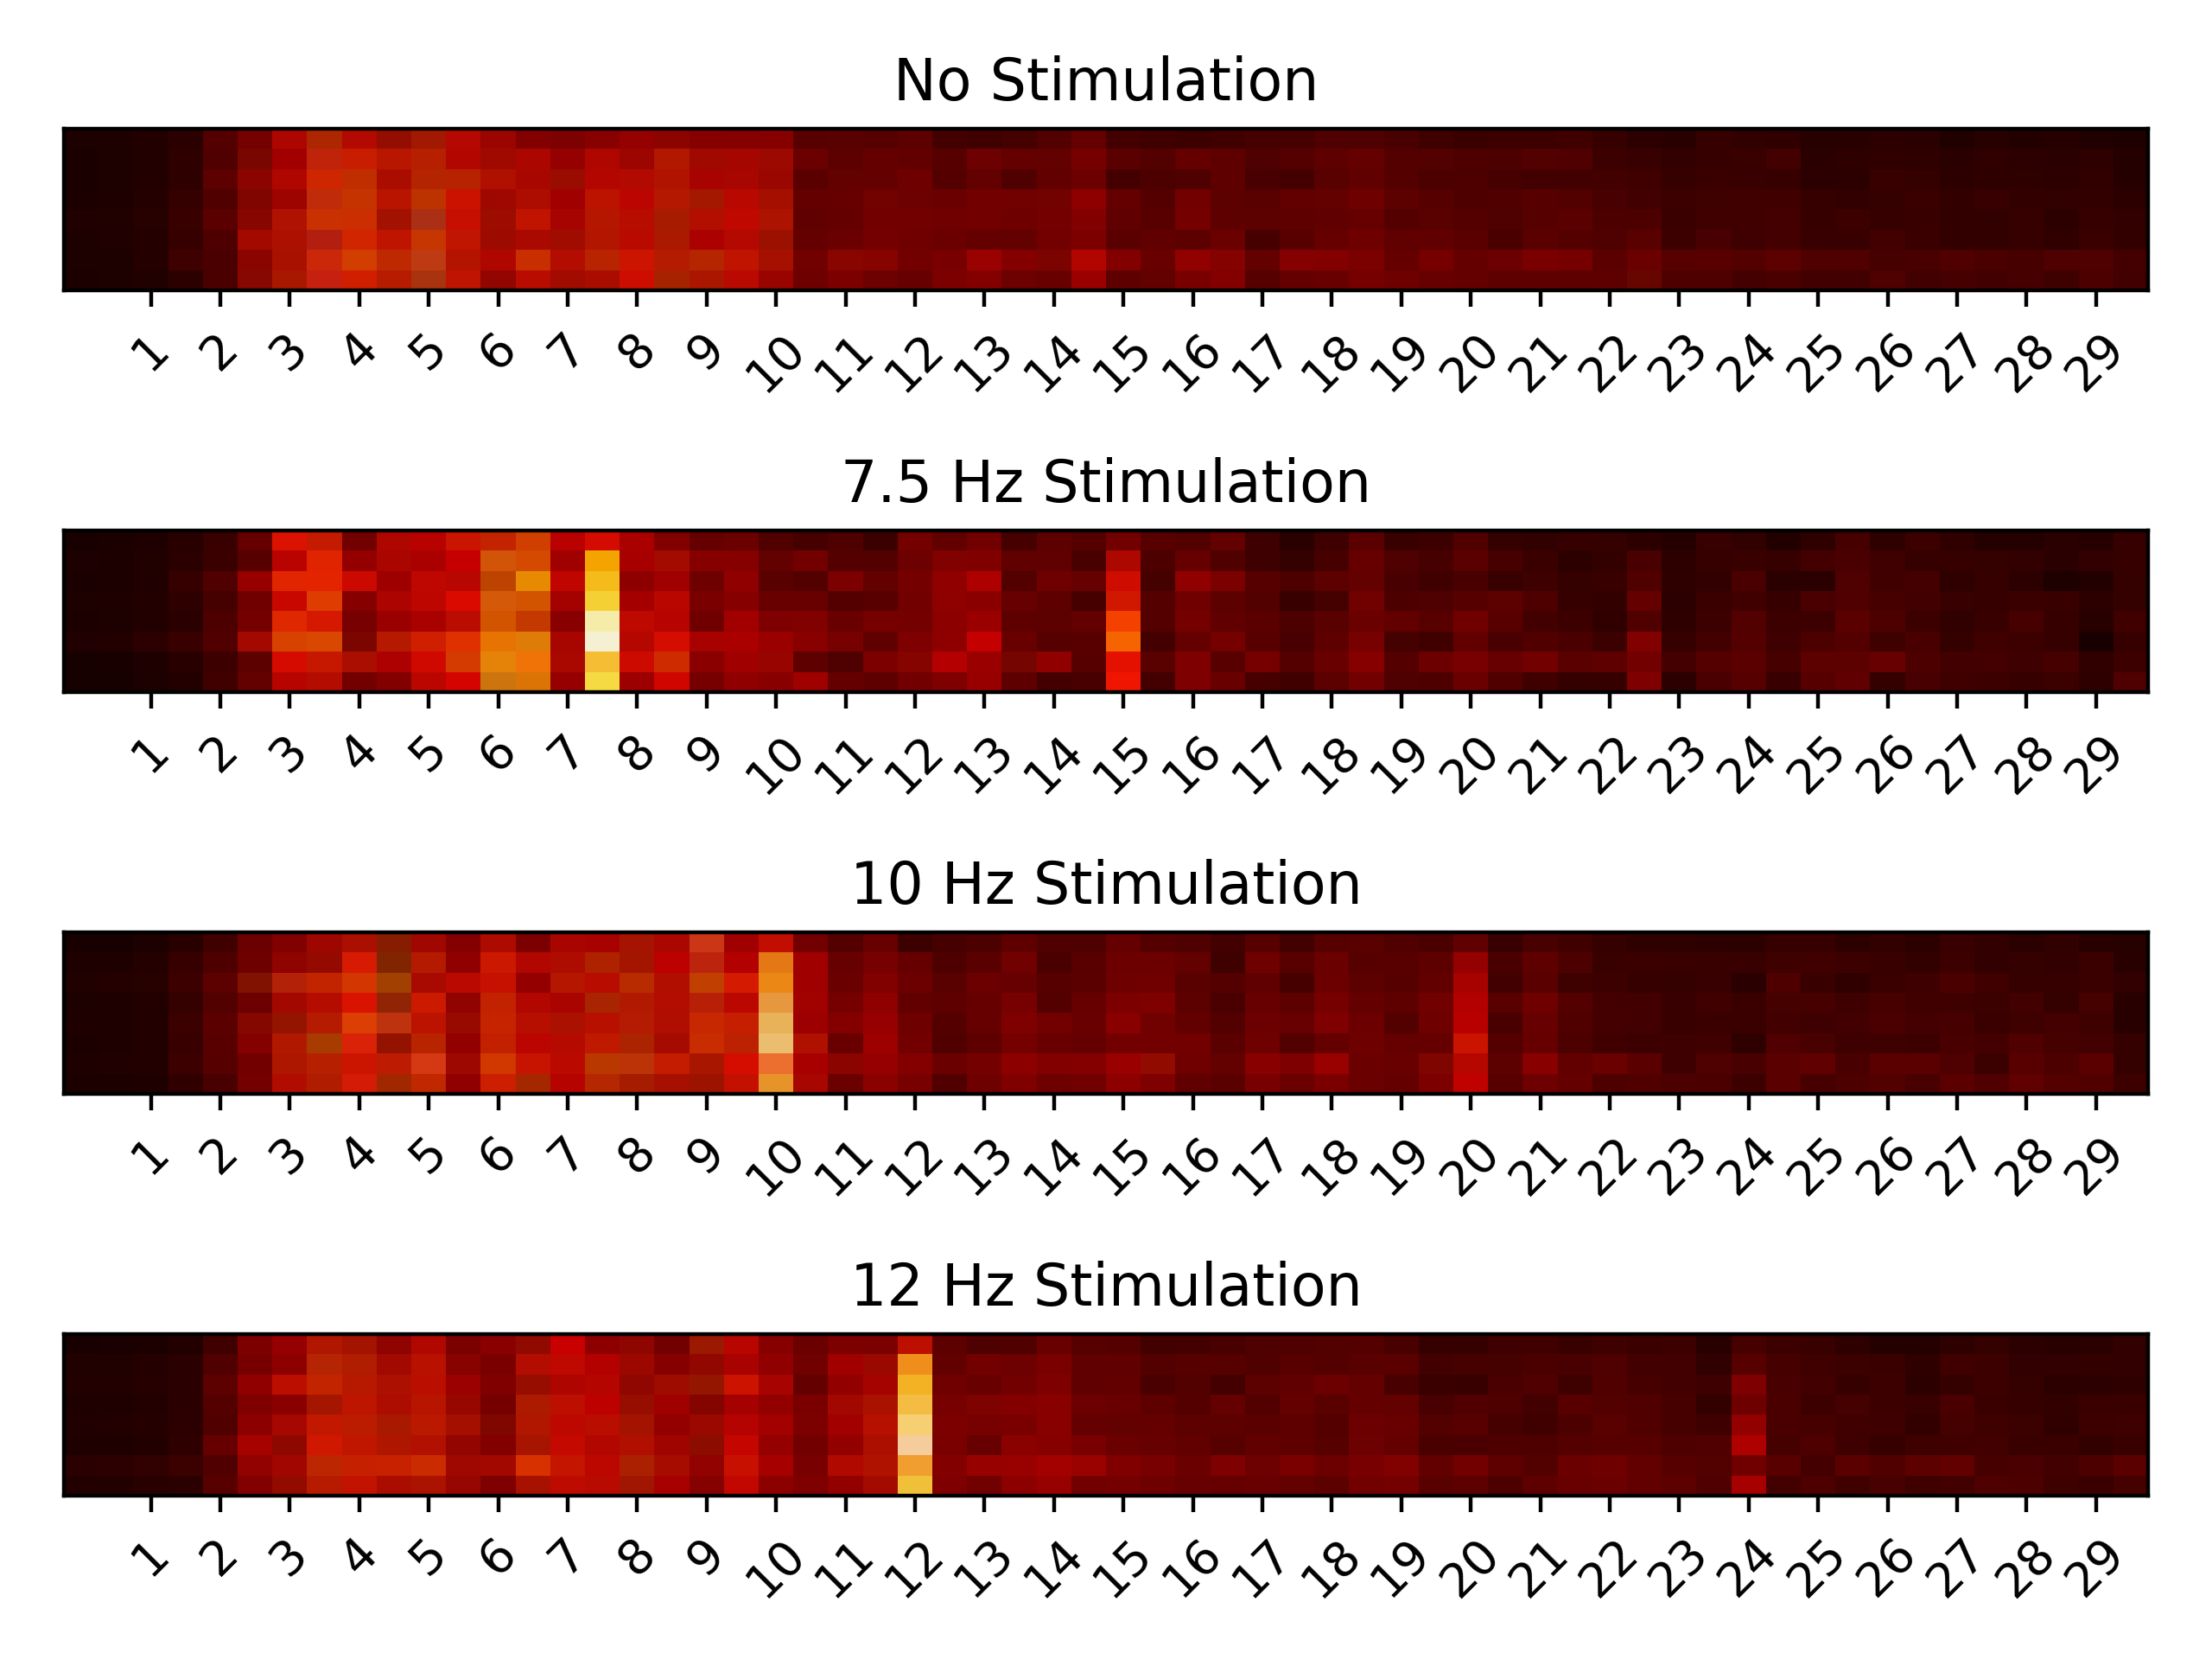
\includegraphics[width=\columnwidth]{images/heatmap.png}
	\end{center}
	
	 The heatmap above shows the average FFT of the time-slices for each channel during the respective stimulation. The light colored stripes show the peaks in the stimulation response. There is also an echo of the response at twice the frequency. It is important to choose frequencies that are not multiples of each other so the signals are clearly distinguishable. 
	 %\smallskip
%\end{flushleft}
}
  

%%%%%%%%%%%%%%%%%%%%%%%%%%%%%%%%%%%%%%%%%%%%%%%%%%%%%%%%%%%%%%%%%%%%%%%%%%%%%%
  \headerbox{Classification}{name=classification,column=2,span=2,row=0}{
%%%%%%%%%%%%%%%%%%%%%%%%%%%%%%%%%%%%%%%%%%%%%%%%%%%%%%%%%%%%%%%%%%%%%%%%%%%%%%
%\begin{flushleft}
 We compared different algorithms to classify time-based EEG-data.
 Steady State Visual Evoked Potentials (SSVEP) is a natural response of the visual cortex evoked by looking at lights flickering at 3.5 to 75~Hz.
 We used the OpenBCI \cite{quelle0} biosensing hardware to record the potentials. Eight of its electrodes were positioned at several locations of the 10-20 system on the back of the head. The time series data were transmitted to a PC at a sample rate of 250~Hz.
 
 The OpenVibe \cite{quelle1} toolkit for brain computer interfaces and real time neurosciences was used to build a data pipeline for the training and classification process. The first pipeline step was filtering the signals with a Butterworth band pass filter (degree=4) between 3 and 40~Hz to reduce the noise of the powergrid at 50~Hz. Subsequently we partitioned the continuous signal into two second time-slices overlapping every 0.2 seconds. The length of the time-slices was chosen so the proceeding Fast Fourier transform has a high enough resolution to differentiate the stimulations (see image of the stimulation response).

 We focused our research on Gaussian Naive Bayes analysis, Support Vector Machines with a polynominal (degree=3) kernel, and Convolutional Neural Networks.
 
Using the Python machine learning package \emph{scikit-learn} \cite{quelle2}, we defined the classifiers as pipeline elements in OpenVibe. The CNN was constructed with \emph{Lasagne}  \cite{quelle3}, a lightweight library to build and train neural networks in \emph{Theano} \cite{quelle4}, together with the \emph{nolearn} \cite{quelle5} wrapper library.

\begin{center}
	\includegraphics[width=\columnwidth]{images/cnn.pdf}
\end{center}

%\end{flushleft}
  }
  
%%%%%%%%%%%%%%%%%%%%%%%%%%%%%%%%%%%%%%%%%%%%%%%%%%%%%%%%%%%%%%%%%%%%%%%%%%%%%%

 \headerbox{Training Session}{name=session,column=0,span=2, below=response}{
%%%%%%%%%%%%%%%%%%%%%%%%%%%%%%%%%%%%%%%%%%%%%%%%%%%%%%%%%%%%%%%%%%%%%%%%%%%%%%
\begin{center}
	%\vspace{0.25cm}
	\includegraphics[width=\columnwidth]{images/session.png}
\end{center}
  }
  
%%%%%%%%%%%%%%%%%%%%%%%%%%%%%%%%%%%%%%%%%%%%%%%%%%%%%%%%%%%%%%%%%%%%%%%%%%%%%%  
  \headerbox{Results}{name=results,column=4,span=2,row=0}{
%%%%%%%%%%%%%%%%%%%%%%%%%%%%%%%%%%%%%%%%%%%%%%%%%%%%%%%%%%%%%%%%%%%%%%%%%%%%%%
 \begin{flushleft}
 	%\smallskip
 	\resizebox{\columnwidth}{!}{
	\begin{tabular}{ l l }
		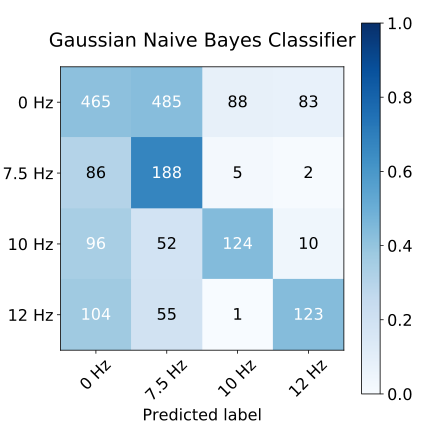
\includegraphics[height=12em]{images/conf_gnb.pdf} & 
		\raisebox{0.05\height}{
			\begin{tabular}[b]{ l l l l l }
				\multicolumn{5}{c}{\textbf{Gaussian Naive Bayes}}\\[1.2ex]
				& precision & recall & f1-score & support \\
	        	class 0     &  0.62  &    0.41  &    0.50   &   1121  \\
		        class 1     &  0.24  &    0.67  &    0.35   &    281  \\
		        class 2     &  0.57  &    0.44  &    0.50   &    282  \\
		        class 3     &  0.56  &    0.43  &    0.49   &    283  \\
		        avg / total & 0.55   &    0.46  &    0.48   &   1967  \\[1.1ex]
		        \multicolumn{5}{l}{Accuracy: 0.45754956787 }\\
			\end{tabular}
		} \\
		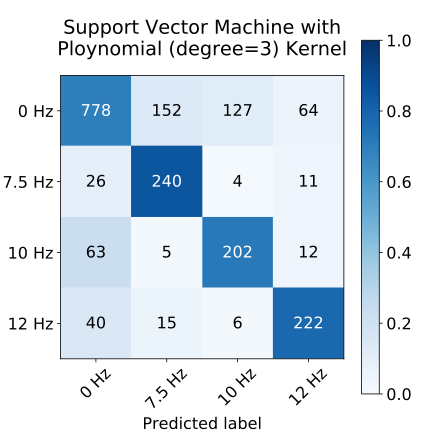
\includegraphics[height=12em]{images/conf_svm.pdf} &
		\raisebox{0.05\height}{
			\begin{tabular}[b]{ l l l l l }
				\multicolumn{5}{c}{\textbf{Support Vector Machine}}\\[1.2ex]
				& precision & recall & f1-score & support \\
				class 0     &  0.86  &    0.69  &    0.77  &  1121  \\
				class 1     &  0.58  &    0.85  &    0.69  &   281  \\
				class 2     &  0.60  &    0.72  &    0.65  &   282  \\
				class 3     &  0.72  &    0.78  &    0.75  &   283  \\
				avg / total &  0.76  &    0.73  &    0.74  &   1967 \\[1.1ex]
				\multicolumn{5}{l}{Accuracy: 0.733096085409 }\\
			\end{tabular}
		} \\
		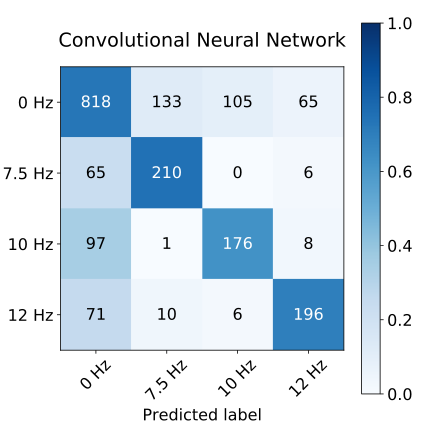
\includegraphics[height=12em]{images/conf_cnn.pdf} & 
		\raisebox{0.05\height}{
			\begin{tabular}[b]{ l l l l l }
				\multicolumn{5}{c}{\textbf{Convolutional Neural Network}} \\[1.2ex]
				& precision & recall & f1-score & support \\
				class 0     & 0.78      & 0.73   & 0.75     & 1121    \\
				class 1     & 0.59      & 0.75   & 0.66     & 281     \\
				class 2     & 0.61      & 0.62   & 0.62     & 282     \\
				class 3     & 0.71      & 0.69   & 0.70     & 283     \\
				avg / total & 0.72      & 0.71   & 0.71     & 1967    \\[1.1ex]
				\multicolumn{5}{l}{Accuracy: 0.711743772242 }\\
			\end{tabular}
		} 
	\end{tabular}
	}

\end{flushleft}
	
	The confusion matrices above visualize the performance of the different algorithms.
	The GNB classifier applies Bayes' Theory with an independence between features assuming a Gaussian distribution of the continuous data.
	
	The SVM divides the features of the different classes through transformation to maximize the margin between the classes. Using a so called \emph{kernel method}, the inputs can be mapped into high-dimensional feature-spaces to perform non-linear classification.
	
	CNN classifiers use convolution operations to extract patterns with high information density from the features and feed them into a fully connected network trained by back-propagation.
 %\end{flushleft}
}

%%%%%%%%%%%%%%%%%%%%%%%%%%%%%%%%%%%%%%%%%%%%%%%%%%%%%%%%%%%%%%%%%%%%%%%%%%%%%%%

\headerbox{References}{name=references,column=2,span=4,row=0.565, below=results}{
%%%%%%%%%%%%%%%%%%%%%%%%%%%%%%%%%%%%%%%%%%%%%%%%%%%%%%%%%%%%%%%%%%%%%%%%%%%%%%%
  
  %\smaller
  \bibliographystyle{ieee}
  \renewcommand{\section}[2]{\vskip 0.05em}
  \begin{thebibliography}{1}\itemsep=-0.01em
  	
  	\setlength{\baselineskip}{0.4em}
  	\bibitem{quelle0} OpenBCI | Low-cost, high-quality biosensing hardware for brain computer interfacing. [Online]. Available: 
  	\url{http://openbci.com/}
  	
        	\setlength{\baselineskip}{0.4em}
        	\bibitem{quelle1} OpenViBE | Software for Brain Computer Interfaces and Real Time Neurosciences. [Online]. Available:\newline
	\url{http://openvibe.inria.fr}

	\setlength{\baselineskip}{0.4em}
        	\bibitem{quelle2} scikit-learn | Machine Learning in Python. [Online]. Available: 
	\url{http://http://scikit-learn.org}
      

	\setlength{\baselineskip}{0.4em}
        	\bibitem{quelle3}Lasagne | Lightweight library to build and train neural networks in Theano . [Online]. Available:\newline
	\url{https://github.com/Lasagne/Lasagne}
      

	\setlength{\baselineskip}{0.4em}
        	\bibitem{quelle4} Theano | evaluate mathematical expressions involving multi-dimensional arrays efficiently. [Online]. Available:\newline
	\url{https://github.com/Theano/Theano}
	
	\setlength{\baselineskip}{0.4em}
	\bibitem{quelle5} nolearn | scikit-learn compatible neural network library. [Online]. Available: 
	\url{https://github.com/dnouri/nolearn}
      
      
  
   \end{thebibliography}
   %\vspace{0.3em}
   
}
    
    
  
    

\end{poster}

\end{document}

